\begin{frame}[label=CTXFigMap]{Regional Map}

\begin{figure}
\centering

\begin{subfigure}{0.48\textwidth}
    \centering
    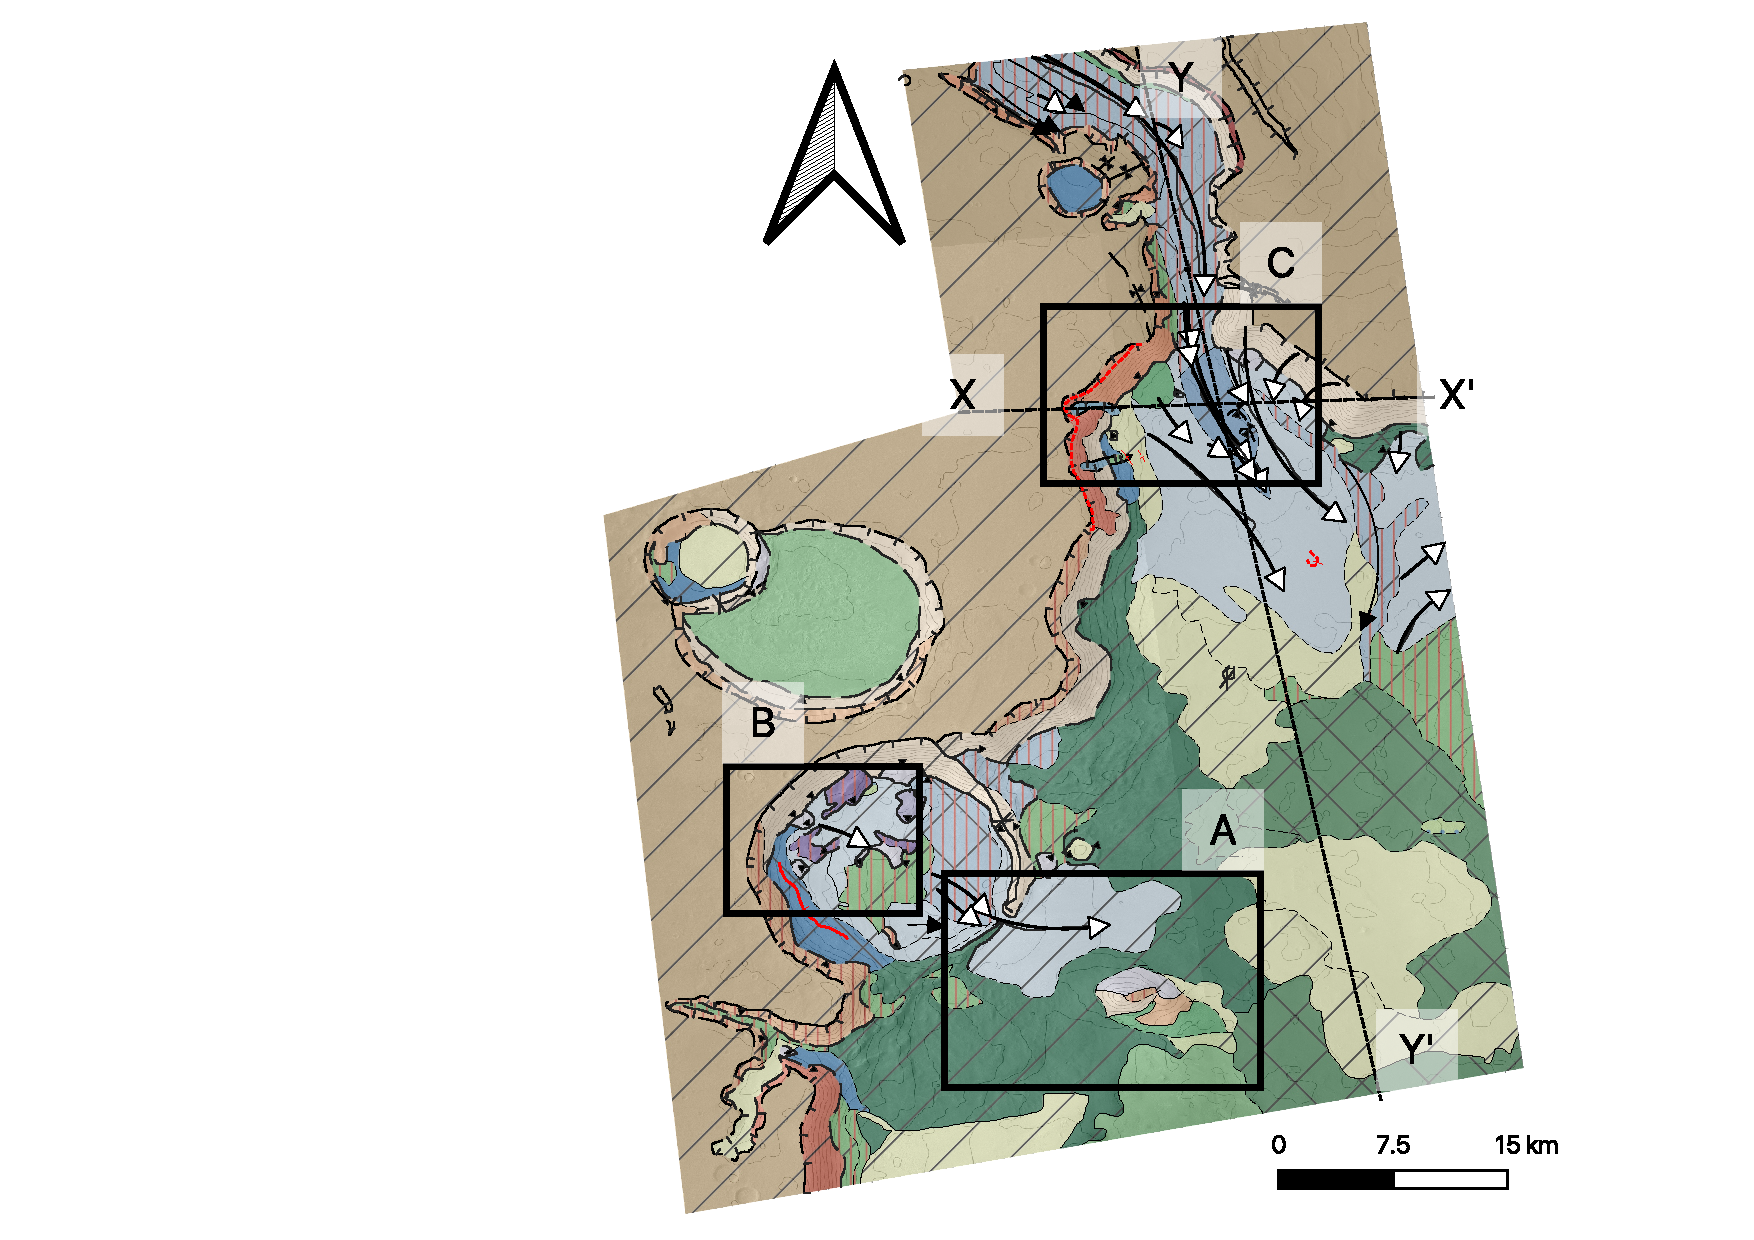
\includegraphics[
        width=\linewidth,
        height=0.65\textheight,
        keepaspectratio
    ]{Figures/Maps/CTX_Final_FigsMap.pdf}
    \label{fig:CTXFinal_a}
\end{subfigure}
\hfill
\begin{subfigure}{0.48\textwidth}
    \centering
    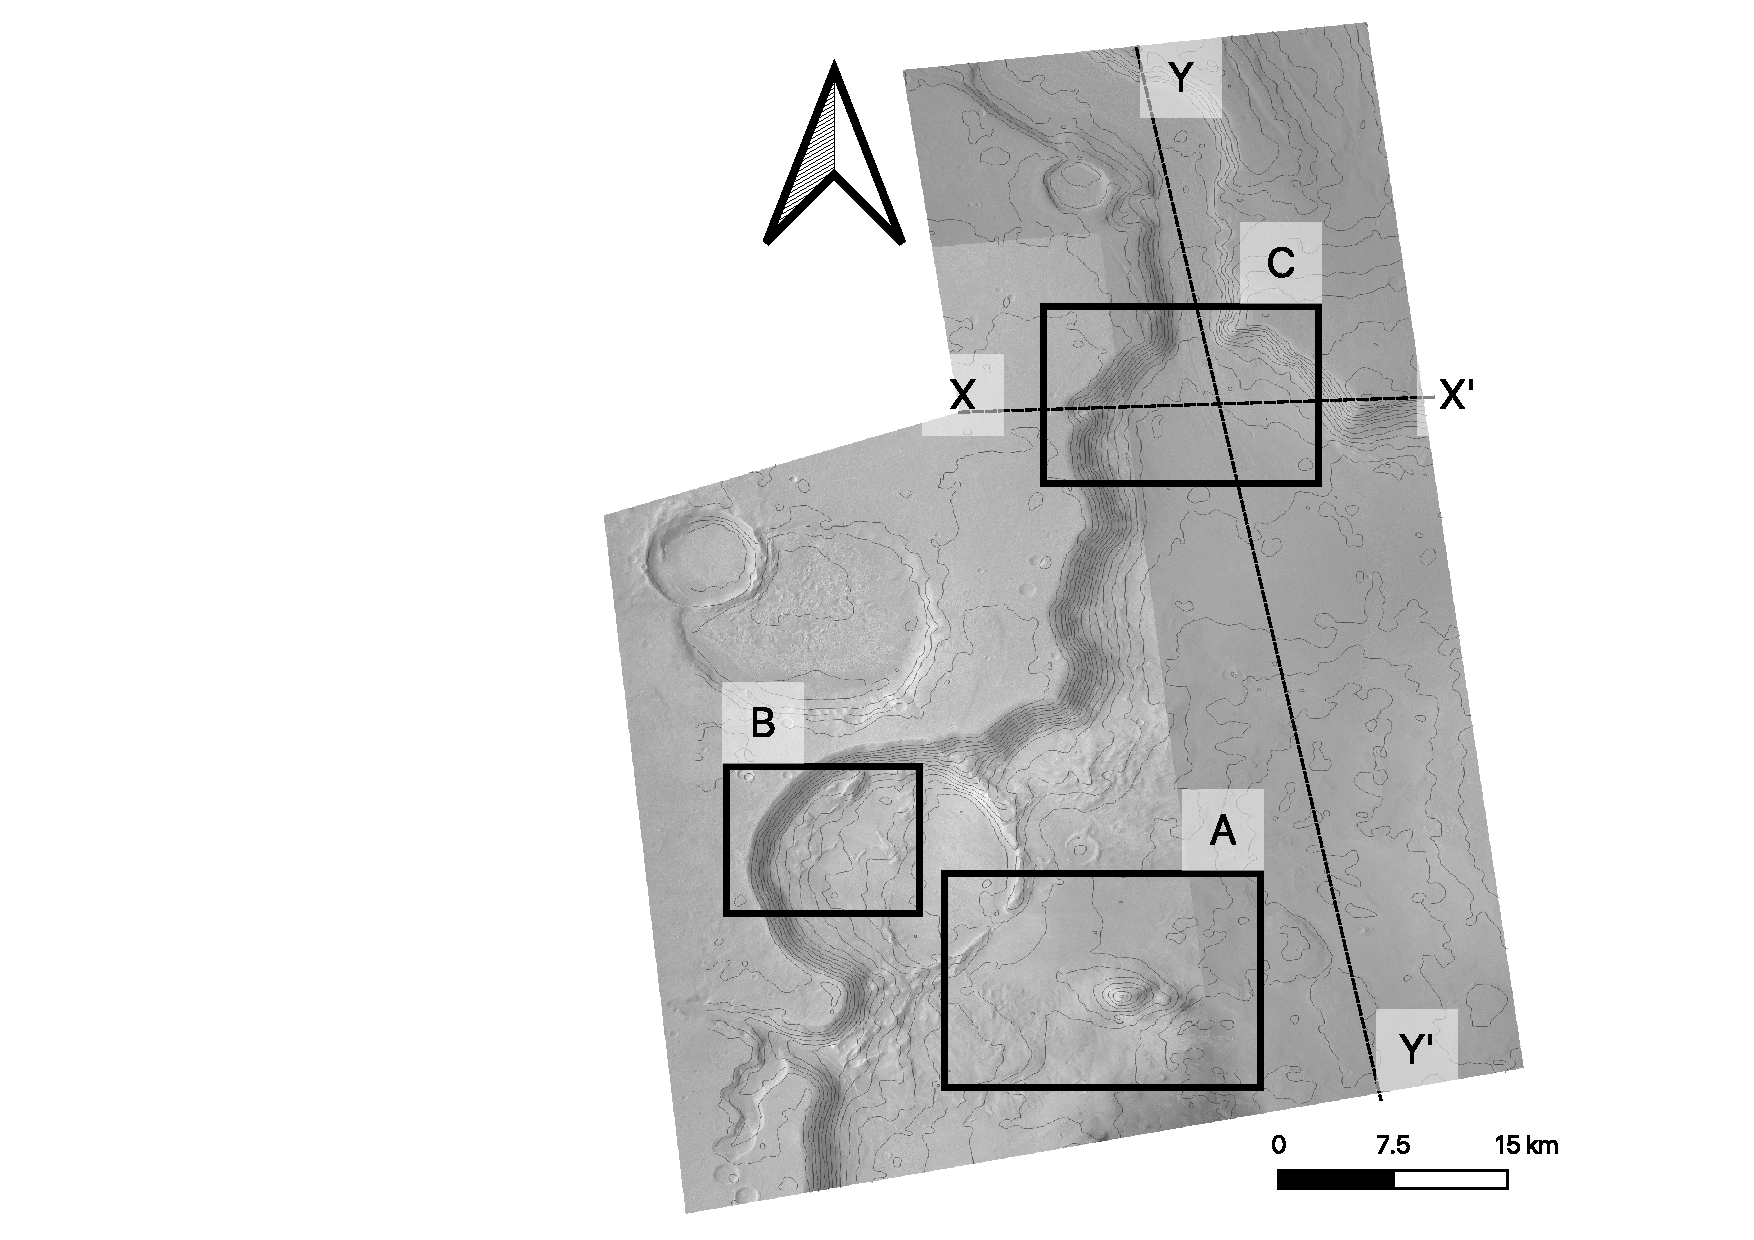
\includegraphics[
        width=\linewidth,
        height=0.65\textheight,
        keepaspectratio
    ]{Figures/Maps/CTX_Final_FigsImg.pdf}
    \label{fig:CTXFinal_b}
\end{subfigure}

\caption{Regional map (from Figure \ref{fig:CTXOverview}) with inserts (A-C; to be shown in alphabetical order) and cross-sections (XX', YY') annotated.}
\label{fig:CTXFinal}
\end{figure}
\end{frame}
